%&exerciseformat.fmt
\documentclass[12pt, a4paper]{article}
\usepackage{exercise}
\usepackage{amsmath}
\usepackage{amsfonts}
\usepackage{mathtools}
\usepackage[shortlabels]{enumitem}
\usepackage[margin=2.5cm]{geometry}
\usepackage{enumitem}
\usepackage{minted}
\usepackage{booktabs}
\usepackage[french]{babel}
\usepackage{graphicx}
\usepackage{caption}
\usepackage{array}
\usepackage{multirow}
\usepackage[symbol]{footmisc}
\usepackage{lmodern} % keep above "fourier" to avoir font change (allows minted text to be displayed as vector)
\usepackage[upright]{fourier}
\usepackage{hhline}
\usepackage{ChkTeX}
%\usepackage{showframe}

\graphicspath{ {./rsc/} }
% New definition of square root:
% it renames \sqrt as \oldsqrt
\let\oldsqrt\sqrt
% it defines the new \sqrt in terms of the old one
\def\sqrt{\mathpalette\DHLhksqrt}
\def\DHLhksqrt#1#2{%
\setbox0=\hbox{$#1\oldsqrt{#2\,}$}\dimen0=\ht0
\advance\dimen0-0.2\ht0
\setbox2=\hbox{\vrule height\ht0 depth -\dimen0}%
{\box0\lower0.64pt\box2}}

\renewcommand{\ExerciseHeader}
{
  \par\noindent
  \textbf{\large \ExerciseName\ \ExerciseHeaderNB\ExerciseHeaderTitle\ExerciseHeaderOrigin}%
  \par\nopagebreak\medskip
}

\renewcommand{\ExerciseName}{Exercice}

\DeclarePairedDelimiter\norm{\lVert}{\rVert}

\def\arraystretch{1.5}

\begin{document}

    \title{Exercices Chapitre sur les Variables Aléatoires\footnote{Page 328 du manuel Hatier}}
    \author{Diego Van Overberghe}
    \maketitle
    
    \begin{Exercise}[number={33}]
        \begin{enumerate}[a)]
          \item $p=1-0{,}34-0{,}26-0{,}17-0{,}12=0{,}11$
          \item $p=1-0{,}26-0{,}24-0{,}14-0{,}13-0{,}04=0{,}19$
        \end{enumerate}
    \end{Exercise}

    \begin{Exercise}[number={35}]
      \begin{enumerate}[a)]
        \item On a: 
              \begin{center}\begin{tabular}{ | l || *{8}{c|} }
                \hline
                $x_i$                     & -1             & 0              & 1              & 3              & 4             & 5             & 6              & 8              \\ \hline
                $P(X=x_i)$ \hspace{0.5cm} & $\frac{1}{20}$ & $\frac{1}{10}$ & $\frac{1}{10}$ & $\frac{3}{20}$ & $\frac{1}{4}$ & $\frac{1}{5}$ & $\frac{1}{10}$ & $\frac{1}{20}$ \\ \hline
               \end{tabular}\end{center}
               \parbox{\linewidth}{\captionof{figure}{Tableau présentant la loi de probabilité de X}}
               
        \item $P(1\leq X\leq 5)=p_1+p_3+p_4+p_5=0{,}1+0{,}15+0{,}25+0{,}2=0{,}7$ \\ $P(X\geq 4)=p_{-1}+p_0+p_1+p_3+p_4=0{,}65$
      \end{enumerate}
    \end{Exercise}

    \begin{Exercise}[number={36}]
      \begin{enumerate}[a)]
        \item On a:
              \begin{center}\begin{tabular}{ | l || *{3}{c|} }
                \hline      
                $x_i$                     & -4            & 0             & 2             \\ \hline
                $P(X=x_i)$ \hspace{0.5cm} & $\frac{1}{9}$ & $\frac{5}{9}$ & $\frac{1}{3}$ \\ \hline
              \end{tabular}\end{center}
              \parbox{\linewidth}{\captionof{figure}{Tableau présentant la loi de probabilité de X}}

        \item On a $x$, le nombre de jetons rouges ou verts et $y$, le nombre de jetons bleus.
              \begin{equation*}
                \begin{cases}2x+y=20\\y=2x\end{cases}\iff\begin{cases}x=5\\y=10\end{cases}
              \end{equation*} \medbreak
              \begin{center}\begin{tabular}{ | l || *{3}{c|} }
                \hline
                $x_i$                     & -4            & 0             & 2             \\ \hline
                $P(X=x_i)$ \hspace{0.5cm} & $\frac{1}{4}$ & $\frac{1}{2}$ & $\frac{1}{4}$ \\ \hline
              \end{tabular}\end{center}
              \parbox{\linewidth}{\captionof{figure}{Tableau présentant la loi de probabilité de X}}

      \end{enumerate}
    \end{Exercise}

    \clearpage

    \begin{Exercise}[number={39}]
      \begin{itemize}
        \item[] On a $p=1-0{,}12-0{,}14-0{,}21-0{,}32-0{,}13=0{,}08$ \medbreak
                De plus, $P(U\leq 13)=0{,}12+0{,}14+0{,}21+0{,}32=0{,}79$ \medbreak
                Donc, $q=P(U\leq 13)-0{,}14-0{,}10=0{,}55$ \medbreak
                Et, $r=1-P(V\leq 13)-0{,}10=0{,}11$
      \end{itemize}
    \end{Exercise}

    \begin{Exercise}[number={40}]
      \begin{enumerate}[a)]
        \item Faux. $P(X\geq 4)=0{,}15$ \medbreak
        \item Faux. $P(2\leq X\leq 3)=0{,}35$ \medbreak
        \item Vrai. $P(X\leq 2)=0{,}15$
      \end{enumerate}
    \end{Exercise}

    \begin{Exercise}[number={50}]
      \begin{enumerate}[a)]
        \item $E(X)=p_0x_0+p_1x_1+p_2x_2+p_3x_3+p_4x_4=1{,}2$ \\ $V(X)=p_0(x_0-E(X))^2+\dots+p_r(x_r-E(X))^2=1{,}46$ \\ $\sigma(X)\approx 1{,}21$
        \item $E(Y)=p_0y_0+\dots+p_ry_r=1{,}1$ \\ $V(Y)=p_0(y_0-E(Y))^2+\dots+p_r(y_r-E(Y))^2=0{,}0184$ \\ $\sigma(Y)\approx 0{,}14$
        \item $E(Z)=p_0z_0+\dots+p_rz_r=1{,}01$ \\ $V(X)=p_0(z_0-E(Z))^2+\dots+p_r(z_r-E(Z))^2\approx 2{,}05$ \\ $\sigma(Z)\approx  1{,}43$
      \end{enumerate}
    \end{Exercise}

    \begin{Exercise}[number={51}]
      \begin{enumerate}[1)]
        \item $E(X)=p_0x_0+\dots+p_rx_r=4{,}9$ \\ $V(X)=p_0(x_0-E(X))^2+\dots+p_r(x_r-E(X))^2=1{,}81$ \\ $\sigma(X)\approx 1{,}35$
        \item \begin{enumerate}[a)]
              \item \ \begin{center}\begin{tabular}{ | l || *{6}{c|} }
                      \hline
                      $y_j$                     & 0      & 1      & 2      & 3     & 4      & 5      \\ \hline
                      $P(Y=y_j)$ \hspace{0.5cm} & 0{,}05 & 0{,}12 & 0{,}18 & 0{,}3 & 0{,}23 & 0{,}12 \\ \hline
                    \end{tabular}\end{center}
                    \parbox{\linewidth}{\captionof{figure}{Tableau présentant la loi de probabilité de Y}}

                    \begin{center}\begin{tabular}{ | l || *{6}{c|} }
                      \hline
                      $z_j$                     & 2{,}4  & 3{,}6  & 4{,}8  & 6     & 7{,}2  & 8{,}4  \\ \hline
                      $P(Z=z_j)$ \hspace{0.5cm} & 0{,}05 & 0{,}12 & 0{,}18 & 0{,}3 & 0{,}23 & 0{,}12 \\ \hline
                    \end{tabular}\end{center}
                    \parbox{\linewidth}{\captionof{figure}{Tableau présentant la loi de probabilité de Z}}

                    \begin{center}\begin{tabular}{ | l || *{6}{c|} }
                      \hline
                      $t_j$                     & 2{,}8  & 3{,}7  & 4{,}6  & 5{,}5 & 6{,}4  & 7{,}3  \\ \hline
                      $P(T=t_j)$ \hspace{0.5cm} & 0{,}05 & 0{,}12 & 0{,}18 & 0{,}3 & 0{,}23 & 0{,}12 \\ \hline
                    \end{tabular}\end{center} 
                    \parbox{\linewidth}{\captionof{figure}{Tableau présentant la loi de probabilité de T}}

              \item \begin{equation*}
                      \begin{aligned}
                        E(Y)&=E(X)-2=2{,}9 \\ V(Y)&=1{,}81 \\ \sigma(Y)&\approx 1{,}35
                      \end{aligned}
                      \hspace{2cm}
                      \begin{aligned}
                        E(Z)&=5{,}88 \\ V(Z)&\approx 2{,}61 \\ \sigma(Z)&=1{,}62
                      \end{aligned}
                      \hspace{2cm}
                      \begin{aligned}
                        E(T)&=5{,}41 \\ V(T)&\approx 1{,}47 \\ \sigma(T)&\approx 1{,}63
                      \end{aligned}
                    \end{equation*}
              \end{enumerate}
      \end{enumerate}
    \end{Exercise}

    \begin{Exercise}[number={52}]
      \begin{enumerate}[a)]
        \item $E(X)=p_0x_0+\dots+p_rx_r=1{,}99$
        \item $E(Y)=p_0y_0+\dots+p_ry_r=2{,}13$
        \item Au centre d'examen B, les candidats font plus d'erreurs en moyenne.
        \item $\sigma(X)=\sqrt{V(X)}=\sqrt{p_0(x_0-E(X))^2+\dots+p_r(x_r-E(X))^2}\approx 1{,}24$ \smallbreak $\sigma(Y)=\sqrt{V(Y)}=\sqrt{p_0(y_0-E(Y))^2+\dots+p_r(y_r-E(Y))^2}\approx 1{,}76$ \smallbreak La centre d'examen B a donc les résultats les plus dispérsés.
      \end{enumerate}
    \end{Exercise}

    \begin{Exercise}[number={56}]
      \begin{enumerate}[a)]
        \item Les représentations graphiques peuvent tous etre assimilées à des paraboles dont le sommet se situe à un abscisse de 25. Donc, les espérances des variables seront identiques. Les courbes sont symmétriques par rapport à la doite d'équation $x=25$.
        \item $\sigma(X)<\sigma(Z)<\sigma(Y)$
      \end{enumerate}
    \end{Exercise}

    \begin{Exercise}[number={60}]
      \begin{itemize}
        \item[] $E(X)=p_0x_0+\dots+p_rx_r$; \quad $V(X)=p_0(x_0-E(X))^2+\dots+p_r(x_r-E(X))^2$; \quad $\sigma(X)=\sqrt{V(X)}$ \bigbreak
      \end{itemize}
      \begin{equation*}
        \begin{aligned}
          E(E_1)&=-0{,}21 \\ V(E_1)&=2{,}2259 \\ \sigma(E_1)&\approx 1{,}49
        \end{aligned}
        \hspace{5cm}
        \begin{aligned}
          E(E_2)&=-0{,}21 \\ V(E_2)&= 1{,}8459 \\ \sigma(E_2)&\approx 1{,}36
        \end{aligned}
      \end{equation*} \bigbreak
      \begin{itemize}
        \item[] La marque modélisée par $E_2$ a une espérance identique à celle de $E_1$, mais l'ecart-type est beacoup plus petit, donc il-y-a moins de risque d'avoir un produit très défectueux.
      \end{itemize}
    \end{Exercise}
    
    \begin{Exercise}[number={61}]
      \begin{enumerate}[a)]
        \item Vrai. $E(aX)=aE(X)$
        \item Faux. $\sigma(X+b)=\sigma(X)$
        \item Vrai. $V(0{,}9X)=0{,}9V(X) \quad \sigma(0{,}9X)=0{,}9\sigma(X)$
      \end{enumerate}
    \end{Exercise}

    \begin{Exercise}
      \begin{equation*}
        \begin{aligned}
          E(X)&= 3{,}105 \\ V(X)&\approx 0{,}51 \\ \sigma(X)&\approx 0{,}72
        \end{aligned}
        \hspace{3cm}
        \begin{aligned}
          E(Y)&=3{,}045 \\ V(Y)&\approx 0{,}38 \\ \sigma(Y)&\approx 0{,}62
        \end{aligned}
        \hspace{3cm}
        \begin{aligned}
          E(Z)&=3{,}28 \\ V(Z)&\approx 0{,}67 \\ \sigma(Z)&\approx 0{,}82
        \end{aligned}
      \end{equation*} \bigbreak
      \begin{enumerate}[a)]
        \item La production Z est la plus dispersée.
        \item La production Z a la masse moyenne la plus élevée.
        \item La production Y est la plus régulière.
      \end{enumerate}
    \end{Exercise}

    \begin{Exercise}[number={64}]
      \begin{enumerate}[a)]
        \item Vrai. Les tirages sont indépendants, donc: $P(B\ ;R)=P(B)\times P(R)=P(R)\times P(B)=P(R\ ;B)$
        \item Faux. Les tirages sont indépendants, donc: $P(R\ ;R)=P^2(R)=\frac{1}{16}$
        \item Vrai. Les tirages sont indépendants, donc: $P(B\ ;B)=P^2(B)=\frac{9}{16}$
      \end{enumerate}
    \end{Exercise}

    \begin{Exercise}[number={65}]
      \begin{enumerate}[a)]
        \item Il-y-a 36 issues possibles.
        \item $P(A)=\frac{1}{6}\times\frac{1}{6}=\frac{1}{36}$ \smallbreak
              $P(B)=\frac{1}{6}+\frac{1}{6}-P(\text{\small{``on obtient deux fois 1''}})=\frac{12}{36}-\frac{1}{36}=\frac{11}{36}$ \smallbreak
              $P(C)=\frac{2}{36}=\frac{1}{18}$ 
      \end{enumerate}
    \end{Exercise}

    \begin{Exercise}[number={66}]
      \begin{enumerate}[1.]
        \item \ \\\parbox{\linewidth}{
                    \centering
                    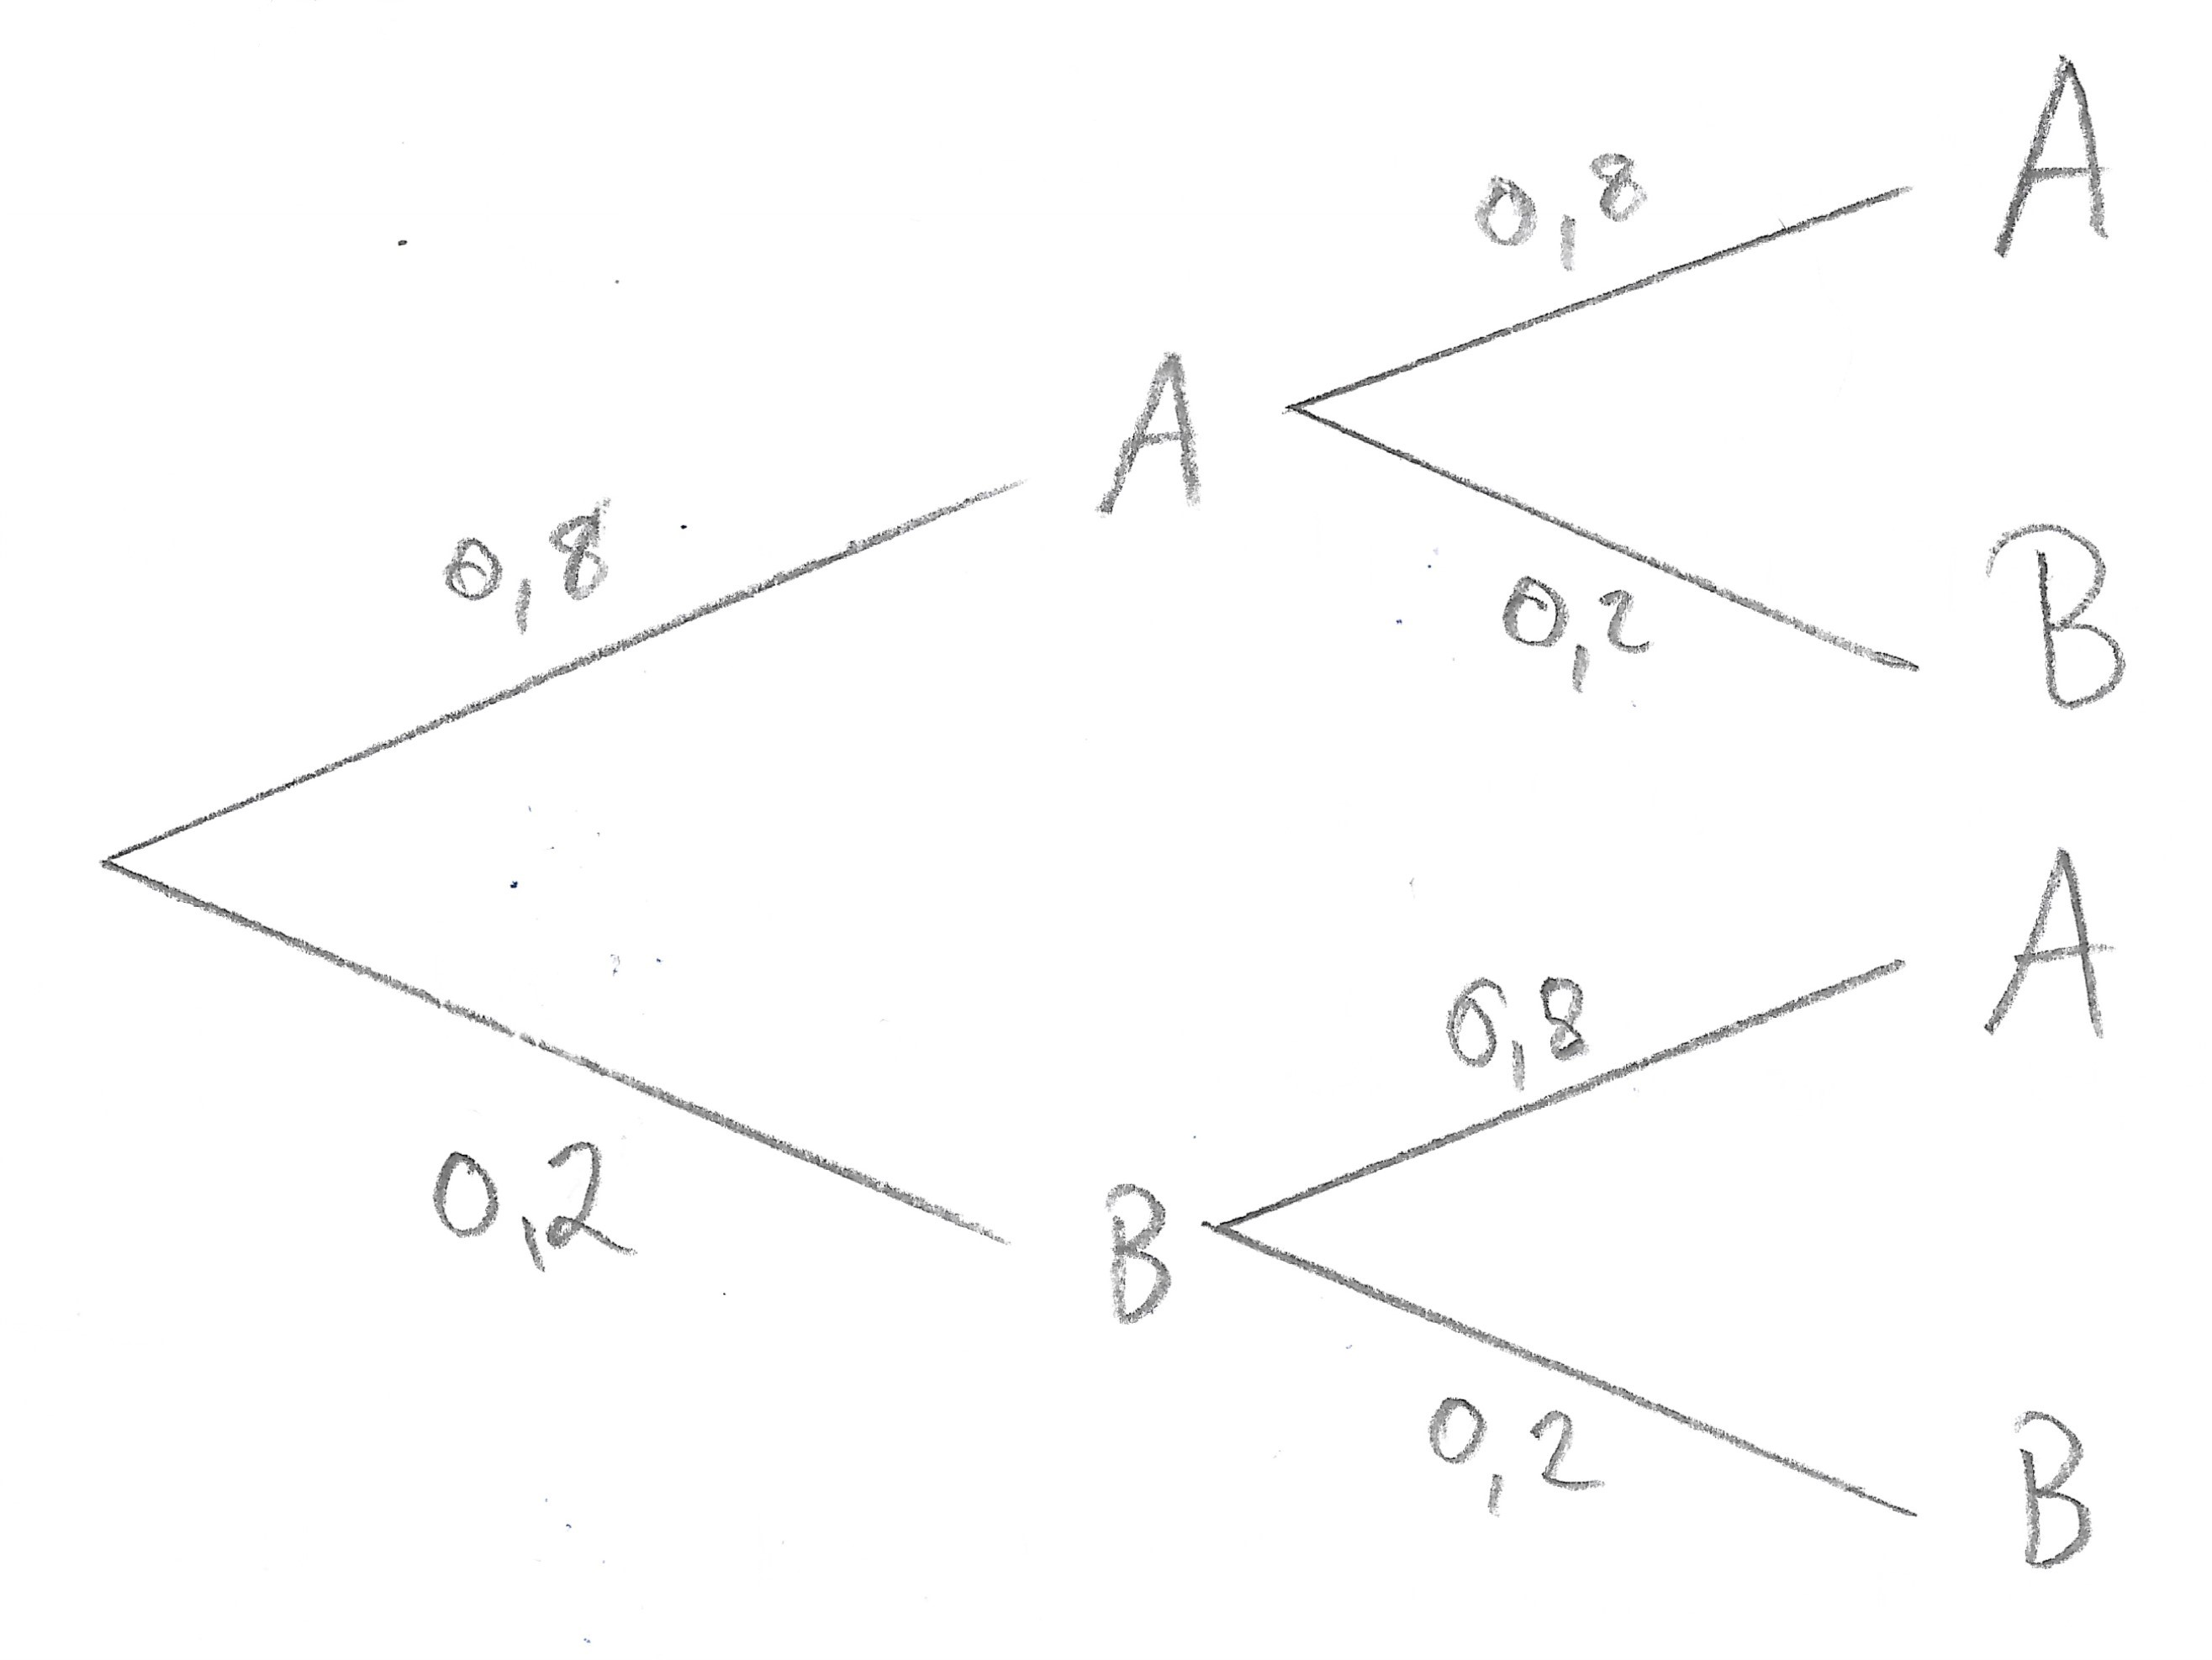
\includegraphics[width=10cm]{VAimg1.jpg}
                    \captionof{figure}{Arbre pondéré}
                  } \bigbreak
        \item \begin{enumerate}[a)]
                \item X prend les valeurs $0$; $1$; $2$.
                \item $P(X=0)=P(\bar{A})^2=\frac{1}{25}$; \quad $P(X=2)=P(A)^2=\frac{16}{25}$ \smallbreak $P(X=1)=1-P(X=0)-P(X=2)=\frac{8}{25}$
                \item $P(X\geq1)=P(X=1)+P(X=2)=\frac{24}{25}$ \smallbreak $P(X\leq1)=P(X=1)+P(X=0)=\frac{9}{25}$
              \end{enumerate}
      \end{enumerate}
    \end{Exercise}

    \begin{Exercise}[number={67}]
      \begin{enumerate}[a)]
        \item L'affirmation de Victor est fausse. Chaque lancer est indépendant pusisque le dé n'est pas truqué. \\ Sa justification est fausse parce que il considère qu'au deuxieme lancer, il n'y a plus que cinq faces, or il y en a toujours six.
        \item Valentine, quand à elle a raison. Il n'y a que $\frac{1}{6}$ de chance que l'un des deux joueurs commencent à jouer au premier tour.
      \end{enumerate}
    \end{Exercise}

    \begin{Exercise}[number={69}]
      \begin{enumerate}[a)]
        \item \ \\\parbox{\linewidth}{
                    \centering
                    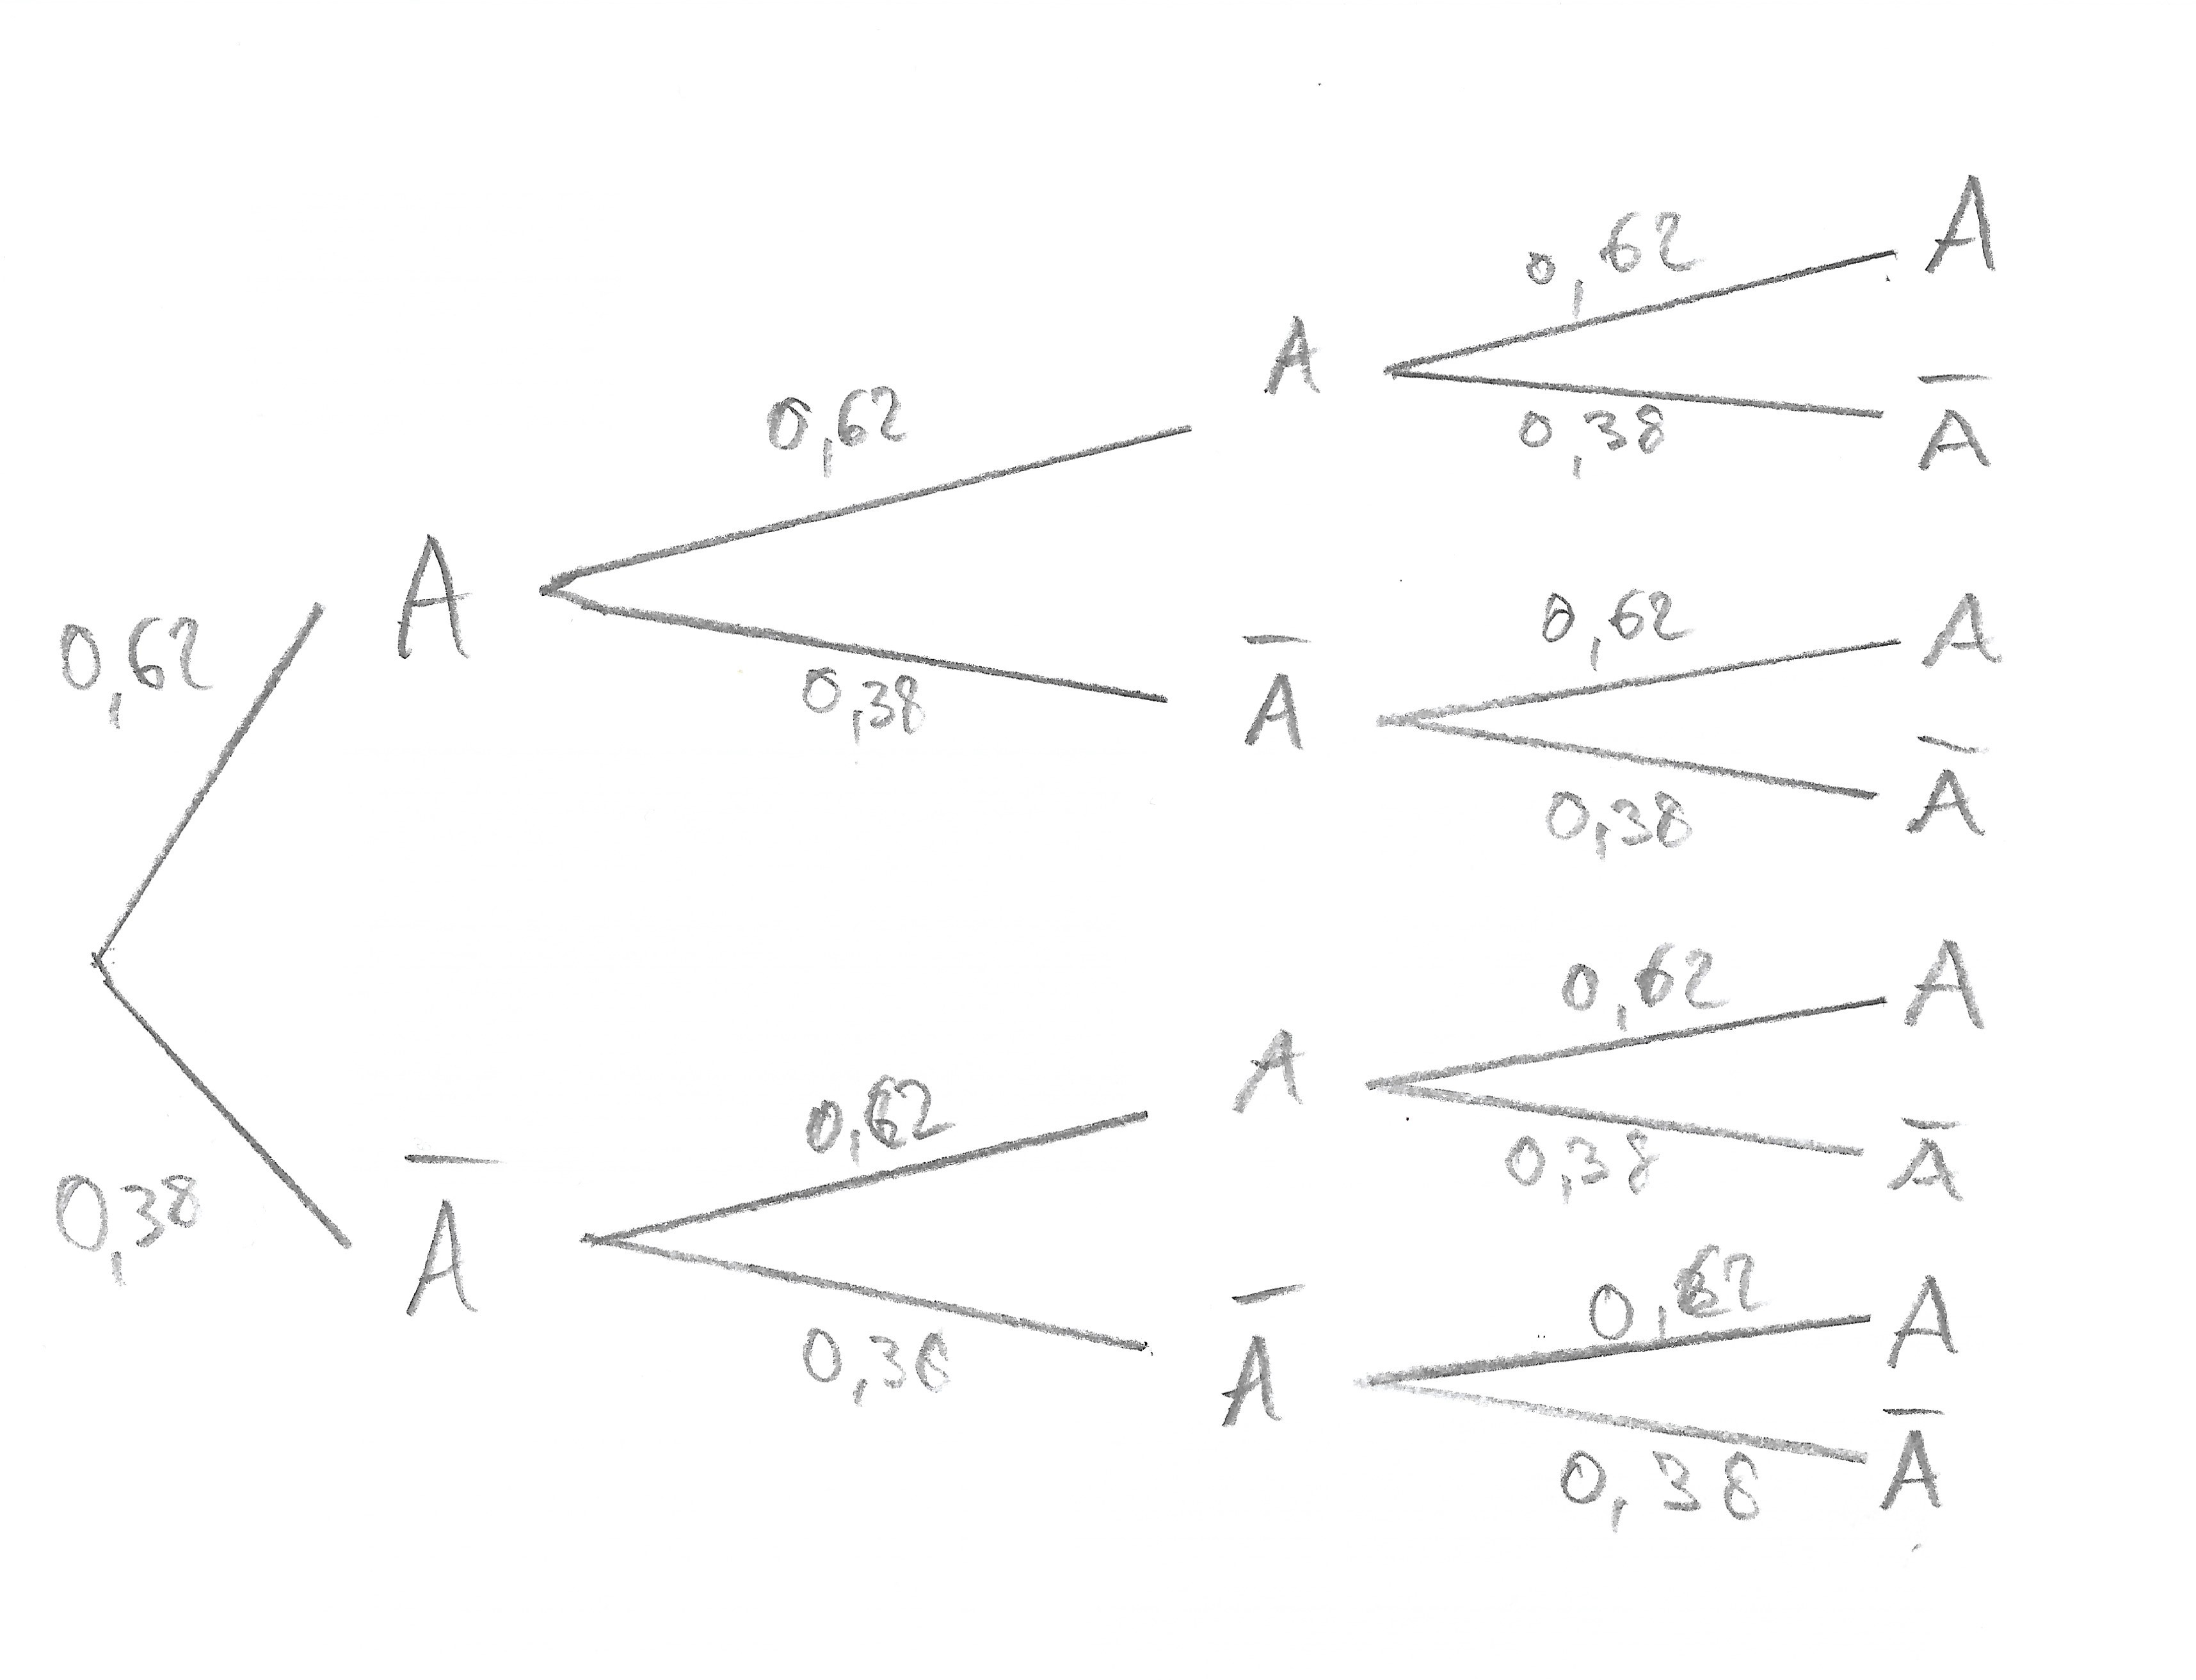
\includegraphics[width=13cm]{VAimg2.jpg}
                    \captionof{figure}{Arbre pondéré}
                  } \bigbreak

        \pagebreak

        \item On pose la variable aléatoire $X$, qui représente le nombre d'usagers abonnés. Ses valeurs possibles sont: $0$; $1$; $2$; $3$. On donne sa loi de probabilité par le tableau ci-dessous, avec \quad $P(X=x_i)=P(\bar{A})^{3-x_i}\times P(A)^{x_i}\times (\text{Nombre d'issues de l'evenement})$
        \begin{center}\begin{tabular}{ |p{0.1\textwidth}||>{\centering}p{0.3\textwidth}|>{\centering\arraybackslash}p{0.3\textwidth}| } \hline
          $x_i$      & 0                                 & 1                                                \\ \hline
          $P(X=x_i)$ & $0{,}38^3\times1\approx 0{,}0549$ & $0{,}38^2\times 0{,}62\times 3\approx 0{,}2686$  \\ \hline\hline
          $x_i$      & 2                                               & 3                                  \\ \hline
          $P(X=x_i)$ & $0{,}38\times 0{,}62^2\times 3\approx 0{,}4382$ & $0{,}62^3\times 1\approx 0{,}2384$ \\ \hline
        \end{tabular}\end{center} \bigbreak
        \parbox{\linewidth}{\captionof{figure}{Tableau présentant la loi de probabilité de X}}

        \begin{itemize}
                \item $P(\text{\small{``Deux des usagers sont abonnés.''}})=P(X=2)\approx0{,}4382$
                \item $P(\text{\small{``Au moins deux des usagers sont abonnés.''}})=P(X\geq2)\approx0{,}6766$
                \item $P(\text{\small{``Au plus deux des usagers sont abonnés.''}})=P(X\leq2)\approx0{,}7617$
              \end{itemize}
        \item \begin{minted}[autogobble]{python}
                import random
                def s_abonnes(nbUsagers=10): # Voir Note 1
                    X=0
                    for ind in range(nbUsagers):
                        if random.random()<0.62:
                            X+=1
                    return X

                print(s_abonnes())

                # Note 1: Il s'agit ici d'un "default parameter", c'est-à-dire que
                # si l'utilisateur ne donne pas d'argument, alors 10 est utilisé.
              \end{minted}
              On cherche quelle est la probabilité que sept des usagers sur les dix soient abonnés. J'utilise la méthode décrite dans le ``Savoir-Faire'' n$^{\circ}$ 4, Page 323. \smallbreak
              Si on imagine l'arbre pondéré qui modélise la situation, on obtient un arbre énorme. La difficulté est de retrouver combien de branches de l'arbre satisfont notre évènement.
              \begin{equation*}
                2^{10}=1024 \quad \text{branches au niveau de la dernière colonne}
              \end{equation*}
              \begin{equation*}
                \sum^{10}_{n=1}\left({2^n}\right)=2048 \quad \text{branches en total}
              \end{equation*} \medbreak
              Dont seulement une petite partie satisfont P(\text{\small{``7 usagers sont abonnés''}}):
              \begin{equation*}
                \frac{10!}{7!\times 3!}=120\footnote[2]{10 niveaux dans l'arbre, avec 7 ``la personne est abonnée'', et 3 ``la personne n'est pas abonnée''.}
              \end{equation*}
              Finallement, on a $P(Y=7)=0{,}62^7\times 0{,}38^3\times 120\approx 0{,}2319$ \\ 
              Ceci est cohérent avec ce que je retrouve dans mes simualtions $(n=10\ 000)$. \\ Cependant, je suis certain qu'il existe  une méthode $\infty$ment plus simple de résoudre le problème, et que ne demande pas au moins une heure de recherche pour pouvoir calculer le nombre de combinations avec répetition possibles... 
      \end{enumerate}
    \end{Exercise}

    \begin{Exercise}[number={71}]
      \begin{enumerate}[a)]
        \item \ \begin{center}\begin{tabular}{|>{\centering}m{0.2\textwidth}||>{\centering}m{0.05\textwidth}|>{\centering}m{0.05\textwidth}|>{\centering}m{0.05\textwidth}|>{\centering\arraybackslash}m{0.05\textwidth}| } \hline
                Numéro sur la face & 1 & 2 & 3 & 4 \\ \hhline{|=#=|=|=|=|}
                1 & 2 & 3 & 4 & 5 \\ \hline
                2 & 3 & 4 & 5 & 6 \\ \hline
                3 & 4 & 5 & 6 & 7 \\ \hline
                4 & 5 & 6 & 7 & 8 \\ \hline
              \end{tabular}\end{center}
              \parbox{\linewidth}{\captionof{figure}{Tableau à double entrée présentant l'ensemble des valeurs prises par \textit{S}}}

        \item \ \begin{center}\begin{tabular}{|l||>{\centering}m{0.05\textwidth}|>{\centering}m{0.05\textwidth}|>{\centering}m{0.05\textwidth}|>{\centering}m{0.05\textwidth}|>{\centering}m{0.05\textwidth}|>{\centering}m{0.05\textwidth}|>{\centering\arraybackslash}m{0.05\textwidth}| } \hline
                  $s_i$ & 2 & 3 & 4 & 5 & 6 & 7 & 8 \\ \hline
                  $P(S=s_i)$ & $\frac{1}{16}$ & $\frac{1}{8}$ & $\frac{3}{16}$ & $\frac{1}{4}$ & $\frac{3}{16}$ & $\frac{1}{8}$ & $\frac{1}{16}$ \\ \hline
                \end{tabular}\end{center}
                \parbox{\linewidth}{\captionof{figure}{Tableau présentant la loi de probabilité de S}}

        \item \begin{itemize}
                \item $P(A)=p_2+p_4+p_6+p_8=0{,}5$ \qquad ou \qquad $P(A)=\frac{8}{16}=0{,}5$                     % Need to fix alignment some time
                \item $P(B)=p_3+p_5+p_7=0{,}5\hphantom{+p_8\ \,}$ \qquad ou \qquad $P(B)=\frac{8}{16}=0{,}5$
                \item $P(C)=p_2+p_4+p_5+p_7+p_8=\frac{11}{16}$\ \ ou \qquad $P(C)=\frac{11}{16}$
                \item $P(D)=p_3=\frac{1}{8}$ \hspace{3cm} \quad ou \qquad $P(C)=\frac{2}{16}$
              \end{itemize} \medbreak
        \item \begin{itemize}
                \item Les deux experiences sont indépendantes, donc $P(A\cap B)=P(A)\times P(B)=0{,}25$
                \item Les deux experiences sont indépendantes, donc $P(\bar{C}\cap\bar{C})=\left(\frac{5}{16}\right)^2=\frac{25}{256}\approx 0{,}0977$
              \end{itemize}
      \end{enumerate}
    \end{Exercise}

    \begin{Exercise}[number={73}]
      \begin{enumerate}[1)]
        \item On définit A:~``L'adhérent a moins de 15 ans.''; B:~``l'adhérent a entre 15 et 25 ans.''; C:~``L'adhérent a entre 26 et 60 ans.''; D: ``L'adhérent a plus de 60 ans.'' \\\parbox{\linewidth}{
                    \centering
                    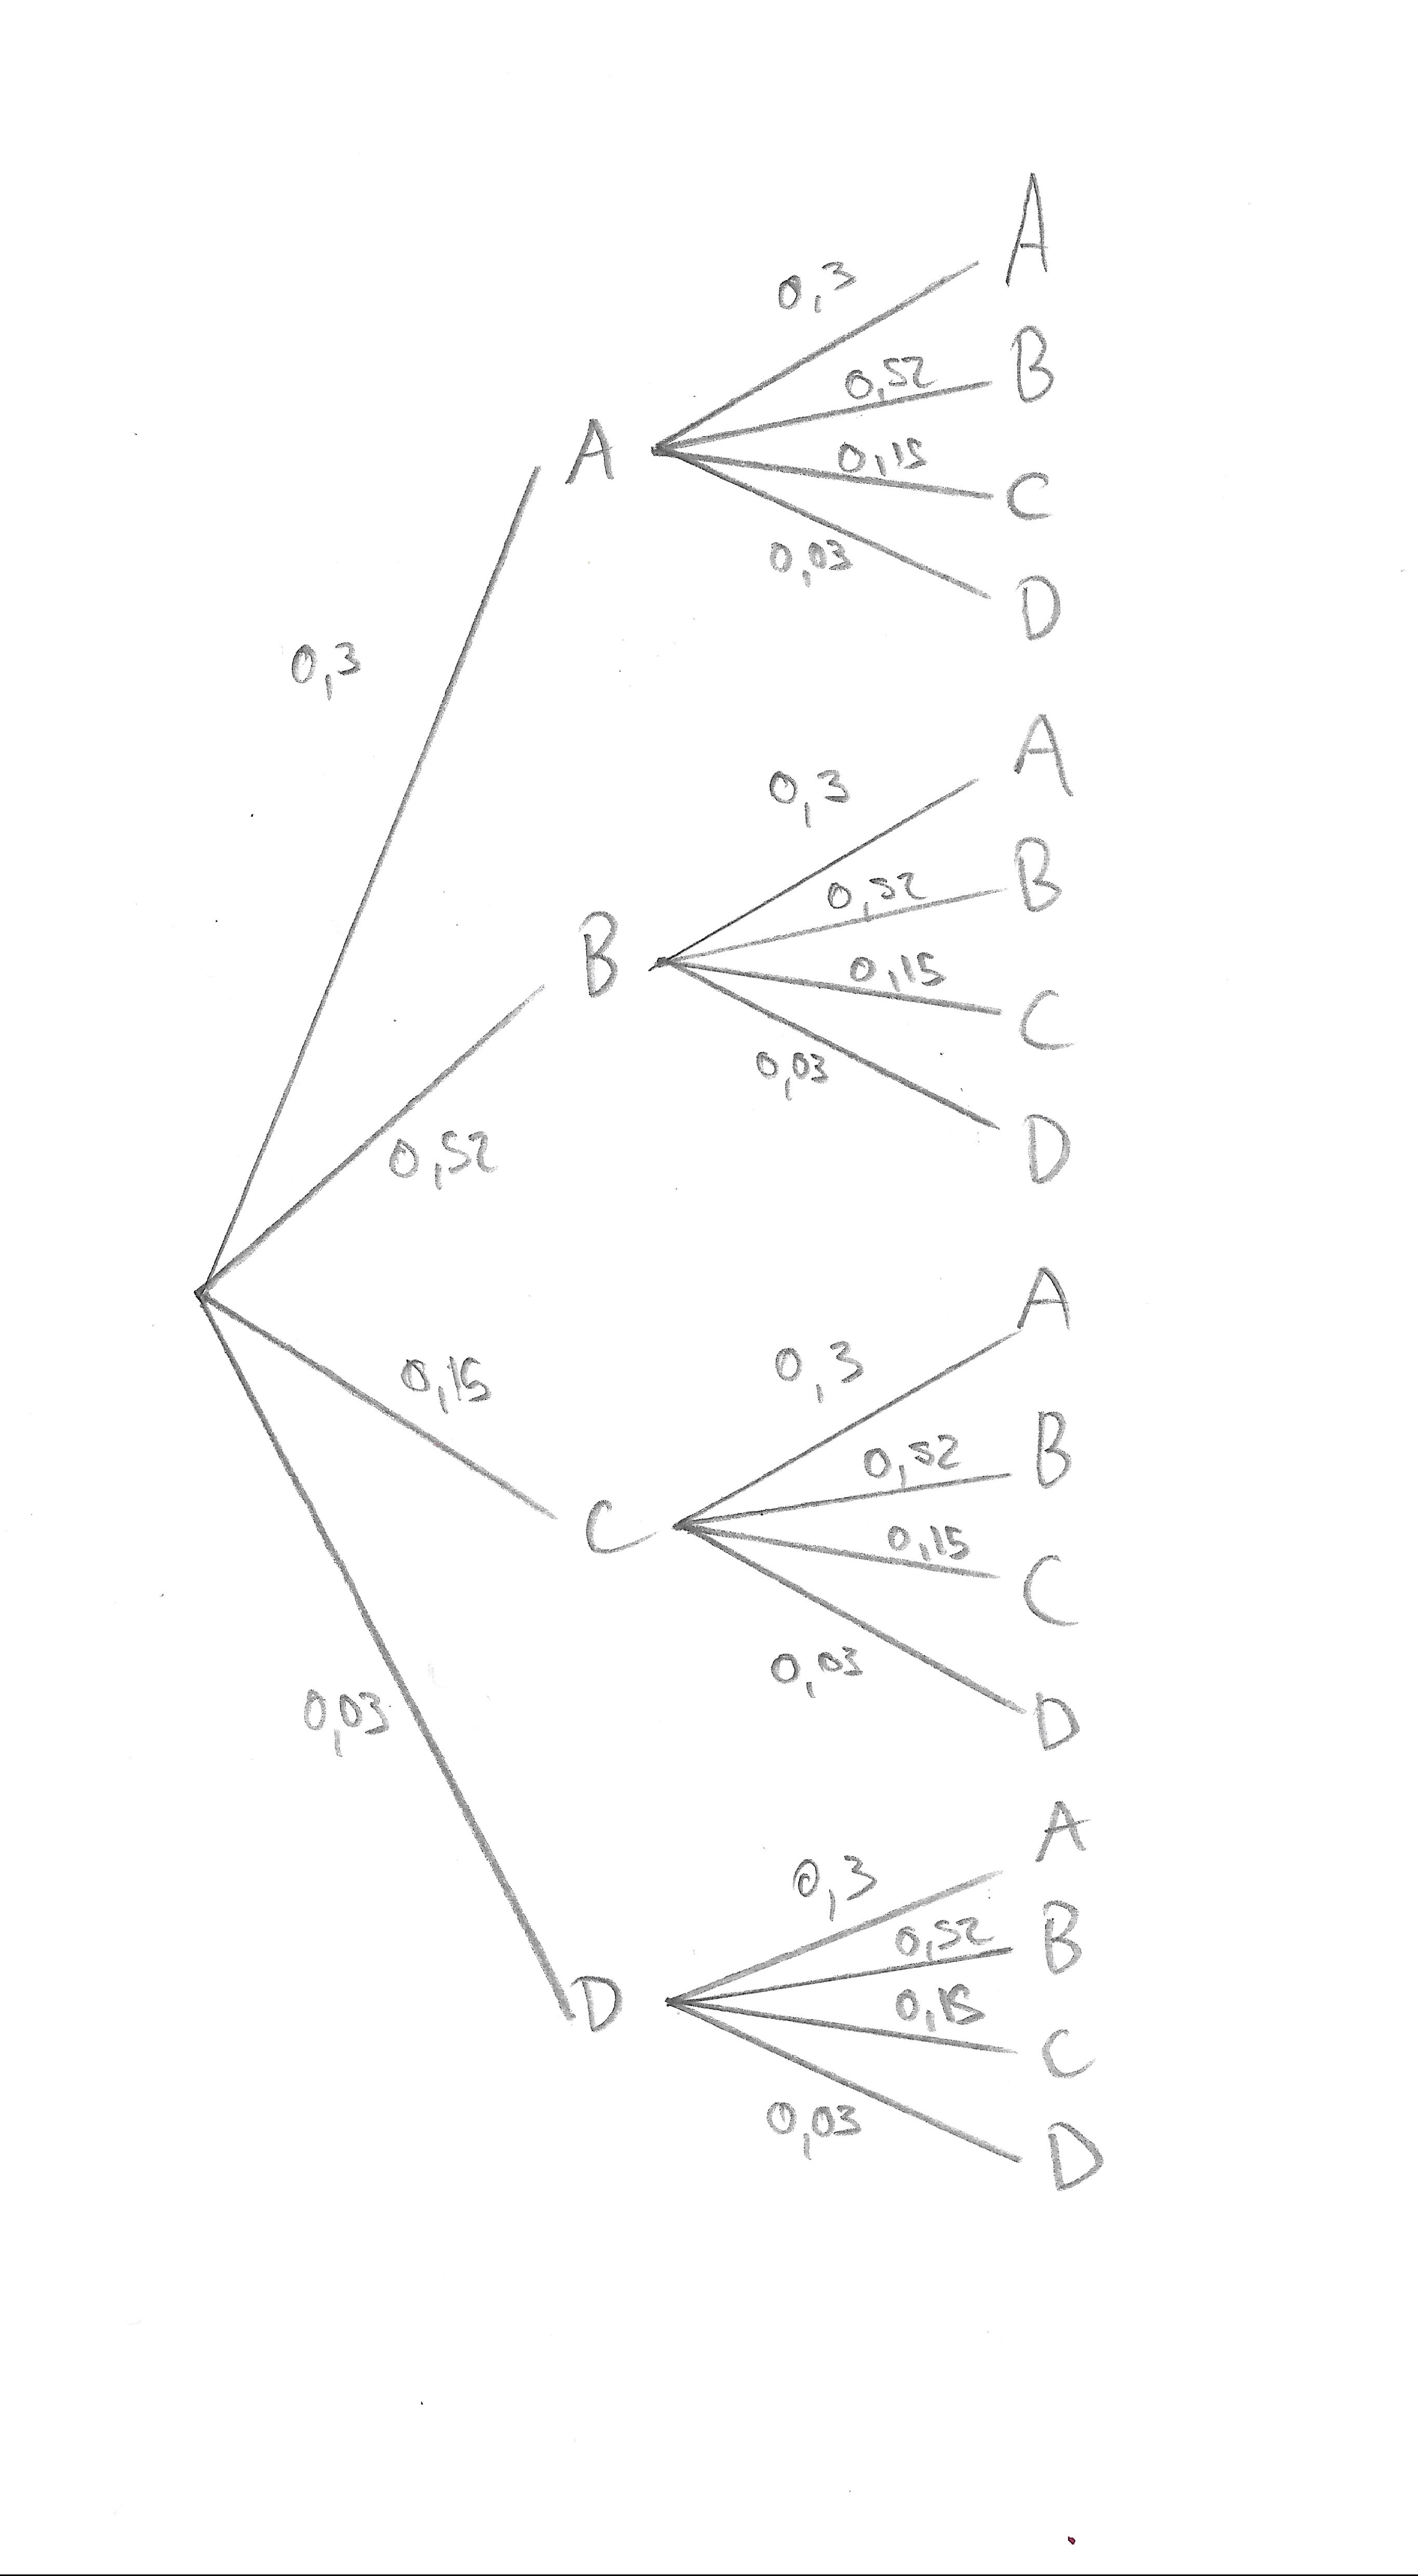
\includegraphics[width=4cm]{VAimg3.jpg}
                    \captionof{figure}{Arbre pondéré}
                  } \bigbreak

        \item Je n'avais pas anticipé le conflit entre les noms des évènements, desormais, les evenements $A$ et $B$ du manuel seront notés $A'$ et $B'$, réspectivement.
              \begin{itemize}
                \item Les réponses sont indépendantes, donc, $P(A')=P(A\cap A)=P(A)^2=0{,}09$
                \item $P(B')=P(D)+P(C\cap D)+P(B\cap D)+P(A\cap D)=0{,}0591$
              \end{itemize} \medbreak
        \item \begin{enumerate}[a)]
                \item $0{,}30^{10}=0{,}000006$
                \item $P(\text{\small{``elles ont tous plus que 60 ans''}})=0{,}03^{10}=6\times 10^{-16}$ \\ D'où $P(\text{\small{``elles n'ont pas tous plus que 60 ans'}})=1-1\times 10^{-16}\approx 0{,}999999$
              \end{enumerate}
      \end{enumerate}
    \end{Exercise}

    \begin{Exercise}
      \begin{enumerate}[a)]
        \item \ \footnotesize{\begin{center}\begin{tabular}{|l||>{\centering}m{0.13\textwidth}|>{\centering}m{0.13\textwidth}|>{\centering}m{0.13\textwidth}|>{\centering}m{0.13\textwidth}|>{\centering\arraybackslash}m{0.13\textwidth}| } \hline
                  $x_i$      & 0                         & 1                                                & 2 & 3 & 4 \\ \hline
                  $P(X=x_i)$ & $0{,}55^4\approx 0{,}092$ & $0{,}55^3\times 0{,}45^1\times 4\approx 0{,}300$ & $0{,}55^2\times 0{,}45^2\times 6\approx 0{,}368$ & $0{,}55^1\times 0{,}45^3\times 4\approx 0{,}200$ & $0{,}45^4\approx 0{,}041$ \\ \hline
                \end{tabular}\end{center}}
                \parbox{\linewidth}{\captionof{figure}{Tableau présentant la loi de probabilité de X}}

        \item $E(X)=p_0x_0+\dots+p_rx_r=1{,}8$ \\ C'est-à-dire qu'en moyenne, 1,8 sur 4, soit 45\%, des femmes agées de 16 ans ou plus, font de l'exercice.
      \end{enumerate}
    \end{Exercise}
\end{document}